\documentclass[lettersize,journal]{IEEEtran}
\usepackage{amsmath,amsfonts}
\usepackage{algorithmic}
\usepackage{array}
\usepackage[caption=false,font=normalsize,labelfont=sf,textfont=sf]{subfig}
\usepackage{textcomp}
\usepackage{stfloats}
\usepackage{url}
\usepackage{verbatim}
\usepackage{graphicx}
\usepackage[english]{babel}

\usepackage{graphicx}
\usepackage{float}
\usepackage{xurl}
\usepackage[hidelinks]{hyperref}
\usepackage[section]{placeins}
\usepackage{booktabs}
\usepackage{multirow}
\usepackage{tikz}
\usetikzlibrary{positioning,arrows.meta}

\emergencystretch=2em
\raggedbottom
\hyphenation{op-tical net-works semi-conduc-tor IEEE-Xplore}
% updated with editorial comments 8/9/2021

\begin{document}

\title{Spectral Feature Selection for Anxiety Detection from EEG Signals in Young Adults}

\author{Jovani Gallegos Álvarez,~\IEEEmembership{Staff,~IEEE,}
        % <-this % stops a space
\thanks{This paper was produced by the IEEE Publication Technology Group. They are in Piscataway, NJ.}% <-this % stops a space
\thanks{Manuscript received April 19, 2021; revised August 16, 2021.}}

% The paper headers
\markboth{Journal of \LaTeX\ Class Files,~Vol.~14, No.~8, August~2021}%
{Shell \MakeLowercase{\textit{et al.}}: A Sample Article Using IEEEtran.cls for IEEE Journals}

\IEEEpubid{0000--0000/00\$00.00~\copyright~2021 IEEE}
% Remember, if you use this you must call \IEEEpubidadjcol in the second
% column for its text to clear the IEEEpubid mark.

\maketitle

\begin{abstract}
Anxiety detection from electroencephalography (EEG) is a clinical and computational challenge. Although EEG provides valuable information, it also contains high redundancy that can affect detection models. This study analyzes several feature selection methods with respect to their ability to remove redundant features and produce more robust anxiety detection models. The work focuses on spectral features extracted from the SAM40 dataset and selected using filter, hybrid, and embedded methods. Results show that feature selection improves the balance between predictive power and interpretability. Experimental findings indicate that the most discriminative features are those extracted from the alpha and delta frequency bands.
\end{abstract}

\begin{IEEEkeywords}
Anxiety, EEG, Feature Selection, mRMR, Fisher, MI.
\end{IEEEkeywords}


\section{Introduction}
\IEEEPARstart{A}{nxiety} disorders represent a significant burden for mental health~\cite{WHOICD11}. In young populations, their academic, social and personal impact is particularly high~\cite{Chand2025}. Although clinical diagnosis through interviews and standardized scales remains essential~\cite{Hamilton1959}, its effectiveness partly depends on self-report and clinician experience~\cite{SCID2018}. In this context, electroencephalography (EEG) combined with machine learning methods offers an objective and non-invasive source for anxiety detection~\cite{StatPearlsEEG2023}.

Anxiety detection from EEG poses an important challenge: spectral, spatial and connectivity features produce high-dimensional spaces with noise and redundancy that significantly affect model performance and interpretability. The physiological signal processing literature has shown that feature selection is a critical step to stabilize classifier performance in high-dimensional spaces~\cite{Acharya2014}. In recent studies using the SAM40 dataset, Afify et al. proposed a CNN for stress detection from EEG and Shikha et al. evaluated stacked classifiers over time- and frequency-domain features~\cite{Afify2025,Shikha2025}.

This study examines several feature selection methods and their ability to identify relevant features that help build more robust and interpretable anxiety detection models. The study focuses on spectral features extracted from the SAM40 dataset~\cite{SAM40Figshare2021} and selected with filter, hybrid and embedded methods.

\section{Methodology}
This section describes the methodological pipeline used in this study: dataset, spectral feature extraction, feature selection, classifier training and evaluation. This pipeline is summarized in Figure~\ref{fig:flujo_metodologia}.

\begin{figure}[H]
	\centering
	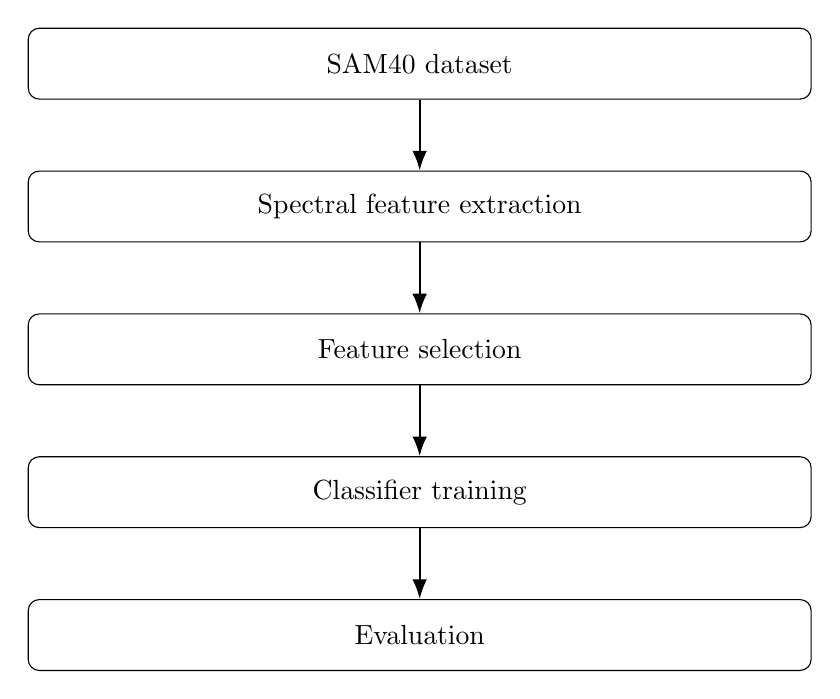
\begin{tikzpicture}[
		node distance=0.9cm,
		box/.style={draw, rounded corners, align=center, minimum width=0.82\linewidth, minimum height=0.9cm},
		arr/.style={-{Latex[length=2.5mm]}, thick}
		]
		\node[box] (d1) {SAM40 dataset};
		\node[box, below=of d1] (d2) {Spectral feature extraction};
		\node[box, below=of d2] (d3) {Feature selection};
		\node[box, below=of d3] (d4) {Classifier training};
		\node[box, below=of d4] (d5) {Evaluation};
		
		\draw[arr] (d1) -- (d2);
		\draw[arr] (d2) -- (d3);
		\draw[arr] (d3) -- (d4);
		\draw[arr] (d4) -- (d5);
	\end{tikzpicture}
	\caption{Main stages of the methodology.\label{fig:flujo_metodologia}}
\end{figure}

\subsection{Dataset}
This study used the SAM40 dataset~\cite{SAM40Figshare2021}, which contains EEG recordings from 40 young participants. Recordings were acquired with a 32-channel Emotiv device at 128 Hz while participants were in a relaxed state and performed three cognitive tasks: a Stroop word-color test, arithmetic problem solving, and symmetric mirror-image identification. Each recording includes a relaxation state and three trials per cognitive task, each lasting 25 seconds.

The dataset also provides the Self-Assessment Manikin (SAM) stress/anxiety score~\cite{Bradley1994} reported after each cognitive task on a 1–10 scale.

\subsection{Feature extraction}
This study focused on the spectral features summarized in Table \ref{tab:resumen_caracteristicas}.
Features were computed over 5 s windows with 50\% overlap. This segmentation increases the number of useful samples while preserving temporal continuity and balancing temporal resolution with spectral stability.

 \begin{table}[!htbp]
	\centering
	\caption{Spectral features, organized by type, considered in this study.}
	\label{tab:resumen_caracteristicas}
	\small
	\renewcommand{\arraystretch}{1.2}
	{\resizebox{\columnwidth}{!}{%
		\begin{tabular}{p{0.24\linewidth} p{0.6\linewidth} c}
			\hline
			Type & Feature & Quantity \\
			\hline
			\multirow{2}{=}{Band power} & alpha, beta & \multirow{2}{*}{160} \\
			& theta, delta, gamma & \\
			\multirow{3}{=}{Hemispheric asymmetries} & Fp2-Fp1, F8-F7, F4-F3, FC6-FC5, & \multirow{3}{*}{50} \\
			& T8-T7, C4-C3 and P8-P7, & \\
			& P4-P3, O2-O1 and PO10-PO9 & \\
			\multirow{2}{=}{Spectral ratios} & theta/beta, theta/alpha & \multirow{2}{*}{96} \\
			& and alpha/beta. & \\
			\hline
			\textbf{Total} & & \textbf{306} \\
			\hline
		\end{tabular}
	}
	}
 \end{table}

For each segment and EEG channel, the power spectral density was estimated using Welch's method. From these estimates, absolute band powers were computed for five bands (alpha, beta, delta, theta, and gamma), yielding 160 spectral features (32 channels × 5 bands).

In addition to band powers, two complementary feature families were extracted: hemispheric asymmetries and spectral ratios. Hemispheric asymmetries were computed for 10 homologous channel pairs: Fp2–Fp1, F8–F7, F4–F3, FC6–FC5, T8–T7, C4–C3, P8–P7, P4–P3, O2–O1 and PO10–PO9. Spectral ratios included theta/beta, theta/alpha and alpha/beta.

Finally, all features were transformed using base-10 logarithm to compress dynamic range, reduce skewness, and improve numerical stability.

\subsection{Feature Selection}
Three feature selection strategies were applied in this study: (i) statistical filter methods, (ii) a hybrid method and (iii) an embedded method.

As filter methods we evaluated the Fisher score (FI) and mutual information (MI), selected for their ability to rank features individually with low computational cost~\cite{Fisher1936}. The Fisher score prioritizes features that maximize between-class separation while minimizing within-class dispersion. Mutual information quantifies how much information each feature provides about the class label, capturing non-linear relationships that linear criteria may miss~\cite{Shannon1948}. The relevance–redundancy framework is supported by information-theoretic foundations for feature selection~\cite{CoverThomas2006}.

mRMR was used as a hybrid method to balance two simultaneous objectives: retaining highly informative features and reducing overlap among similar features (minimum redundancy). This is particularly relevant in EEG, where different channels or bands can contain partially redundant information~\cite{Peng2005}. As an embedded method, feature importance derived from Decision Trees (DT) was used, providing a classifier-dependent non-linear perspective and facilitating interpretation of individual feature contributions~\cite{Breiman2001}. Tree-based models naturally support direct interpretations of relative feature contributions via hierarchical partitioning~\cite{Breiman1984}.


\subsection{Classifier training}
Classification was formulated as a binary problem and evaluated using five classifiers: Decision Tree (DT), Random Forest (RF), k-Nearest Neighbors (KNN), Support Vector Machine (SVM) and XGBoost (XGB). DT and RF provide structural interpretability and feature importance analysis; RF additionally increases robustness through ensembling and reduces variance compared to a single tree. KNN and SVM were included as comparative references: KNN for its simplicity based on local neighborhoods and SVM for its ability to model non-linear boundaries in reduced feature spaces. In particular, SVM serves as a solid reference for assessing the effect of feature selection~\cite{Cortes1995}. Finally, XGBoost makes it possible to assess the impact of feature selection in a boosting model, which combines multiple weak learners into a strong one and often improves classification performance.

For classifier training, we used the dataset summarized in Table \ref{tab:registros}. This dataset was built from feature vectors extracted from the relaxation state and from cognitive tasks where participants reported a stress/anxiety level greater than or equal to 5. Feature vectors from the relaxation state were labeled as Class 0, and those from the cognitive tasks as Class 1.

\FloatBarrier

\begin{table}[!htbp]
	\centering
	\caption{Dataset summary used for building anxiety detection models.}
	\label{tab:registros}
	\small
	\renewcommand{\arraystretch}{1.5}
	\resizebox{\columnwidth}{!}{%
	\begin{tabular}{p{0.38\linewidth} p{0.4\linewidth} c}
	\hline
		\textbf{Dataset} & \textbf{Class} & \textbf{Total per class} \\
	\hline
	\multirow{2}{=}{2508 records $\times$ 306 features} & Class 0: Relaxation & 1080 \\
	& Class 1: Anxiety & 1428 \\
	\hline
	\end{tabular}
}
\end{table}

\FloatBarrier

Before classifier construction, and in order to control interindividual variability and focus the comparison on relative changes with respect to each participant's relaxation state, the dataset was normalized using the Z-score transform according to the mean and standard deviation of the relaxation class.

\subsection{Evaluation}
To evaluate classifier performance and preserve independence among samples from the same participant, leave-one-subject-out cross-validation (LOSO) was used. In each iteration, one entire subject was reserved for testing and the remaining subjects were used for training.

Classifier performance was assessed using three main metrics: sensitivity, specificity and accuracy. These metrics were computed from the confusion matrix accumulated during LOSO validation, where $TP$ denotes true positives, $TN$ true negatives, $FP$ false positives and $FN$ false negatives.

Sensitivity (S) quantifies the model's ability to correctly detect anxiety cases:
\begin{equation}
	\mathrm{Sensitivity}=\frac{TP}{TP+FN}.
\end{equation}

Specificity (E) quantifies the ability to correctly recognize the relaxation class:
\begin{equation}
	\mathrm{Specificity}=\frac{TN}{TN+FP}.
\end{equation}

Accuracy (A) summarizes the overall proportion of correct classifications:
\begin{equation}
	\mathrm{Accuracy}=\frac{TP+TN}{TP+TN+FP+FN}.
\end{equation}

\section{Results}
To evaluate the impact of the selection methods on classifier performance, two experiments were conducted:

\begin{itemize}
	\item Experiment 1: Impact of feature selection on global classifiers.
	\item Experiment 2: Impact of feature selection on specialized classifiers.
\end{itemize}


The experiments were implemented in Python using the \texttt{pandas}, \texttt{NumPy}, \texttt{SciPy}, \texttt{scikit-learn}, \texttt{Matplotlib} and \texttt{Seaborn} libraries. They were run on a MacBook Pro with an Apple M4 processor and 16 GB of RAM.

In addition, the evaluated training configurations were: DT with maximum depth 5 and balanced weighting; RF with 100 trees, balanced weighting and parallel execution; KNN with 5 neighbors; SVM with an RBF kernel and balanced weighting; and XGB with 200 trees, maximum depth 3, learning rate 0.05 and balanced weighting.

\subsection{Experiment 1. Impact of feature selection on global classifiers}
This experiment aims to analyze the effect on classifier performance when using feature subsets of different sizes obtained with Fisher, Mutual Information (MI), minimum Redundancy Maximum Relevance (mRMR) and Decision Trees (DT) selection methods. Specifically, the top 15, 20 and 30 features obtained by these methods were analyzed. This strategy was used to evaluate classifier robustness under dimensionality reduction and to identify more compact feature configurations that do not imply a significant loss of predictive power. This type of analysis is consistent with model evaluation practices in high-dimensional and complex settings~\cite{Goodfellow2016}.

Tables \ref{tab:comp_global} and \ref{tab:comp_global_extra} present classifier performance when using the top 30 (Top-30), 20 (Top-20) and 15 (Top-15) features obtained by Fisher, MI, mRMR and DT selection methods. Table \ref{tab:comp_global} reports model accuracy, while Table \ref{tab:comp_global_extra} summarizes sensitivity and specificity. The results show that the most effective feature selection method is the decision-tree-based one (DT), followed by MI and mRMR. In particular, DT, KNN and XGB achieve their best performance with Top-15, while SVM and RF perform best with Top-20. It is worth noting that SVM and RF achieve slightly lower performance using Top-15, which indicates that DT helps generate sparser models. In addition, the results show that MI and mRMR can produce RF and XGB models with acceptable performance using Top-30.
\FloatBarrier

\begin{table}[!htbp]
	\centering
	\caption{Accuracy attained by models using the top 15 (Top-15), 20 (Top-20) and 30 (Top-30) features selected by Fisher, MI, mRMR and DT.}
	\label{tab:comp_global}
	\scriptsize
	\setlength{\tabcolsep}{1.5pt}
	\renewcommand{\arraystretch}{1}
	\resizebox{\columnwidth}{!}{%
		\begin{tabular}{lccccccccccc}
			\toprule
			\multirow{2}{*}{\textbf{Models}} & \multicolumn{3}{c}{\textbf{Fisher}} & \multicolumn{3}{c}{\textbf{MI}} & \multicolumn{3}{c}{\textbf{mRMR}} & \multicolumn{2}{c}{\textbf{DT}} \\
			\cmidrule(lr){2-4}\cmidrule(lr){5-7}\cmidrule(lr){8-10}\cmidrule(lr){11-12}
			& Top-15 & Top-20 & Top-30 & Top-15 & Top-20 & Top-30 & Top-15 & Top-20 & Top-30 & Top-15 & Top-20 \\
			\midrule
			DT & 0.659 & 0.690 & 0.686 & 0.727 & 0.703 & 0.711 & 0.705 & 0.702 & 0.709 & \textbf{0.745} & 0.744 \\
			KNN & 0.668 & 0.673 & 0.680 & 0.689 & 0.691 & 0.685 & 0.696 & 0.691 & 0.685 & \textbf{0.726} & 0.697 \\
			SVM & 0.720 & 0.734 & 0.746 & 0.768 & 0.770 & 0.785 & 0.760 & 0.770 & 0.785 & \textbf{0.805} & 0.808 \\
			RF & 0.725 & 0.738 & 0.748 & 0.767 & 0.768 & 0.793 & 0.763 & 0.764 & 0.789 & 0.811 & \textbf{0.816} \\
			XGB & 0.719 & 0.725 & 0.748 & 0.772 & 0.776 & 0.784 & 0.774 & 0.782 & 0.785 & \textbf{0.805} & 0.799 \\
			\bottomrule
		\end{tabular}%
	}
\end{table}

\begin{table}[!htbp]
	\centering
	\caption{Sensitivity and specificity attained by models using the top 15 (Top-15), 20 (Top-20) and 30 (Top-30) features selected by Fisher, MI, mRMR and DT.}
	\label{tab:comp_global_extra}
	\scriptsize
	\setlength{\tabcolsep}{1.5pt}
	\renewcommand{\arraystretch}{1}
	\resizebox{\columnwidth}{!}{%
		\begin{tabular}{llccccccccccc}
			\toprule
			\multirow{2}{*}{\textbf{Models}} & \multirow{2}{*}{\textbf{Metric}} & \multicolumn{3}{c}{\textbf{Fisher}} & \multicolumn{3}{c}{\textbf{MI}} & \multicolumn{3}{c}{\textbf{mRMR}} & \multicolumn{2}{c}{\textbf{DT}} \\
			\cmidrule(lr){3-5}\cmidrule(lr){6-8}\cmidrule(lr){9-11}\cmidrule(lr){12-13}
			& & Top-15 & Top-20 & Top-30 & Top-15 & Top-20 & Top-30 & Top-15 & Top-20 & Top-30 & Top-15 & Top-20 \\
			\midrule
			\multirow{2}{*}{DT} & S & 0.525 & 0.536 & 0.532 & 0.567 & 0.527 & 0.555 & 0.536 & 0.525 & 0.553 & 0.596 & 0.595 \\
			& E & 0.838 & 0.893 & 0.890 & 0.939 & 0.936 & 0.918 & 0.928 & 0.936 & 0.915 & 0.943 & 0.940 \\
			\midrule
			\multirow{2}{*}{KNN} & S & 0.574 & 0.563 & 0.552 & 0.588 & 0.597 & 0.546 & 0.605 & 0.597 & 0.546 & 0.601 & 0.539 \\
			& E & 0.793 & 0.819 & 0.849 & 0.823 & 0.815 & 0.869 & 0.817 & 0.815 & 0.869 & 0.892 & 0.906 \\
			\midrule
			\multirow{2}{*}{SVM} & S & 0.616 & 0.637 & 0.648 & 0.665 & 0.672 & 0.698 & 0.659 & 0.672 & 0.698 & 0.730 & 0.739 \\
			& E & 0.858 & 0.862 & 0.876 & 0.904 & 0.899 & 0.899 & 0.894 & 0.899 & 0.899 & 0.903 & 0.899 \\
			\midrule
			\multirow{2}{*}{RF} & S & 0.716 & 0.726 & 0.732 & 0.739 & 0.744 & 0.779 & 0.740 & 0.736 & 0.769 & 0.795 & 0.812 \\
			& E & 0.737 & 0.753 & 0.769 & 0.805 & 0.800 & 0.813 & 0.794 & 0.800 & 0.815 & 0.831 & 0.821 \\
			\midrule
			\multirow{2}{*}{XGB} & S & 0.667 & 0.665 & 0.688 & 0.709 & 0.715 & 0.727 & 0.716 & 0.721 & 0.729 & 0.751 & 0.744 \\
			& E & 0.788 & 0.805 & 0.828 & 0.856 & 0.856 & 0.859 & 0.851 & 0.863 & 0.860 & 0.876 & 0.872 \\
			\bottomrule
		\end{tabular}%
	}
\end{table}

\FloatBarrier



\FloatBarrier
\begin{figure}[!htbp]
	\centering
	
\includegraphics[width=\columnwidth]{\detokenize{Figuras y tablas/Top20_DT_RF.png}}
	\caption{Relative importance of the top 20 features (Top-20) obtained by DT.}
	\label{fig:top20_dt_rf}
\end{figure}
\FloatBarrier

In summary, features selected by DT enabled the construction of anxiety detection models with the best performance. The top 20 features selected by DT, according to their relative importance, are shown in Figure~\ref{fig:top20_dt_rf}.

\subsection{Experiment 2. Impact of feature selection on specialized classifiers}
This experiment evaluates how different feature selection methods affect the performance of classifiers specialized by feature type (bands and derived families). Four selection methods are compared (Fisher, MI, mRMR and DT) in terms of their ability to build two types of detection models: a base model using 32 features and a comparison model using the top 8 features identified by each selection method.

Tables~\ref{tab:comp_alpha}, \ref{tab:comp_beta} and \ref{tab:comp_delta} present results for specialized models on the alpha, beta and delta bands, respectively. These tables report performance for the base models using all available band features (Top-32) and for the comparison models using the top 8 features selected by each method (Top-8).

Results indicate that the best base models for the alpha band were obtained with XGB. mRMR identified the top 8 alpha-band features, enabling sparser models. For the beta band, Table~\ref{tab:comp_beta} shows that the best base models also correspond to XGB, and that DT selection produced sparser models across classifiers. Notably, mRMR identified the top 8 features for beta, which produced the best XGB model. For delta, Table~\ref{tab:comp_delta} indicates that XGB yields the best base models and that DT and mRMR produce sparser Top-8 models without large performance losses.

In summary, the best specialized models were obtained for the alpha and delta bands, using mRMR-selected features for alpha and DT-selected features for delta. The top 8 features identified by mRMR for alpha are shown in Figure~\ref{fig:top8_mrmr_alpha}, while the top 8 identified by DT for delta are shown in Figure~\ref{fig:top8_dt_delta}.

\begin{table}[!htbp]
	\centering
	\caption{Performance achieved by specialized models for the alpha band.}
	\label{tab:comp_alpha}
	\scriptsize
	\setlength{\tabcolsep}{3pt}
	\renewcommand{\arraystretch}{1}
	\resizebox{\columnwidth}{!}{%
		\begin{tabular}{llcccccccc}
			\toprule
			\multirow{2}{*}{\textbf{Models}} & \multirow{2}{*}{\textbf{Metric}} & \multicolumn{2}{c}{\textbf{Fisher}} & \multicolumn{2}{c}{\textbf{MI}} & \multicolumn{2}{c}{\textbf{mRMR}} & \multicolumn{2}{c}{\textbf{DT}} \\
			\cmidrule(lr){3-4}\cmidrule(lr){5-6}\cmidrule(lr){7-8}\cmidrule(lr){9-10}
			& & Top-32 & Top-8 & Top-32 & Top-8 & Top-32 & Top-8 & Top-32 & Top-8 \\
			\midrule
			\multirow{3}{*}{DT} & A & 0.622 & 0.617 & 0.620 & 0.648 & 0.620 & \textbf{0.653} & 0.621 & 0.648 \\
			& S & 0.398 & 0.474 & 0.396 & 0.461 & 0.397 & 0.450 & 0.398 & 0.434 \\
			& E & 0.919 & 0.806 & 0.916 & 0.894 & 0.916 & 0.921 & 0.916 & 0.931 \\
			\midrule
			\multirow{3}{*}{KNN} & A & 0.652 & 0.615 & 0.652 & 0.652 & 0.652 & \textbf{0.662} & 0.652 & 0.656 \\
			& S & 0.532 & 0.568 & 0.532 & 0.618 & 0.532 & 0.584 & 0.532 & 0.605 \\
			& E & 0.812 & 0.677 & 0.812 & 0.697 & 0.812 & 0.765 & 0.812 & 0.724 \\
			\midrule
			\multirow{3}{*}{SVM} & A & 0.740 & 0.650 & 0.740 & 0.693 & 0.740 & \textbf{0.712} & 0.740 & 0.707 \\
			& S & 0.661 & 0.534 & 0.661 & 0.600 & 0.661 & 0.618 & 0.661 & 0.599 \\
			& E & 0.845 & 0.805 & 0.845 & 0.816 & 0.845 & 0.835 & 0.845 & 0.850 \\
			\midrule
			\multirow{3}{*}{XGB} & A & 0.779 & 0.684 & 0.779 & 0.714 & 0.779 & \textbf{0.748} & 0.779 & 0.740 \\
			& S & 0.770 & 0.685 & 0.770 & 0.709 & 0.769 & 0.711 & 0.769 & 0.712 \\
			& E & 0.791 & 0.683 & 0.791 & 0.721 & 0.791 & 0.796 & 0.792 & 0.778 \\
			\bottomrule
		\end{tabular}%
	}
	\end{table}

\begin{table}[!htbp]
	\centering
	\caption{Performance achieved by specialized models for the beta band.}
	\label{tab:comp_beta}
	\scriptsize
	\setlength{\tabcolsep}{3pt}
	\renewcommand{\arraystretch}{1}
	\resizebox{\columnwidth}{!}{%
		\begin{tabular}{llcccccccc}
			\toprule
			\multirow{2}{*}{\textbf{Models}} & \multirow{2}{*}{\textbf{Metric}} & \multicolumn{2}{c}{\textbf{Fisher}} & \multicolumn{2}{c}{\textbf{MI}} & \multicolumn{2}{c}{\textbf{mRMR}} & \multicolumn{2}{c}{\textbf{DT}} \\
			\cmidrule(lr){3-4}\cmidrule(lr){5-6}\cmidrule(lr){7-8}\cmidrule(lr){9-10}
			& & Top-32 & Top-8 & Top-32 & Top-8 & Top-32 & Top-8 & Top-32 & Top-8 \\
			\midrule
			\multirow{3}{*}{DT} & A & 0.625 & 0.616 & 0.625 & 0.618 & 0.626 & 0.604 & 0.625 & \textbf{0.653} \\
			& S & 0.482 & 0.504 & 0.482 & 0.397 & 0.482 & 0.352 & 0.482 & 0.464 \\
			& E & 0.815 & 0.765 & 0.815 & 0.911 & 0.815 & 0.936 & 0.815 & 0.903 \\
			\midrule
			\multirow{3}{*}{KNN} & A & 0.633 & 0.596 & 0.633 & 0.624 & 0.633 & 0.635 & 0.633 & \textbf{0.644} \\
			& S & 0.539 & 0.571 & 0.539 & 0.583 & 0.539 & 0.578 & 0.539 & 0.615 \\
			& E & 0.757 & 0.630 & 0.757 & 0.678 & 0.757 & 0.710 & 0.757 & 0.683 \\
			\midrule
			\multirow{3}{*}{SVM} & A & 0.705 & 0.645 & 0.705 & 0.648 & 0.705 & \textbf{0.689} & 0.705 & 0.677 \\
			& S & 0.584 & 0.488 & 0.584 & 0.505 & 0.584 & 0.557 & 0.584 & 0.550 \\
			& E & 0.865 & 0.852 & 0.865 & 0.837 & 0.865 & 0.864 & 0.865 & 0.844 \\
			\midrule
			\multirow{3}{*}{XGB} & A & 0.775 & 0.690 & 0.777 & 0.700 & 0.776 & \textbf{0.727} & 0.776 & 0.724 \\
			& S & 0.772 & 0.698 & 0.774 & 0.712 & 0.773 & 0.699 & 0.773 & 0.720 \\
			& E & 0.780 & 0.681 & 0.780 & 0.685 & 0.781 & 0.764 & 0.781 & 0.730 \\
			\bottomrule
		\end{tabular}%
	}
	\end{table}


\begin{table}[!htbp]
	\centering
	\caption{Performance achieved by specialized models for the delta band.}
	\label{tab:comp_delta}
	\scriptsize
	\setlength{\tabcolsep}{3pt}
	\renewcommand{\arraystretch}{1}
	\resizebox{\columnwidth}{!}{%
		\begin{tabular}{llcccccccc}
			\toprule
			\multirow{2}{*}{\textbf{Models}} & \multirow{2}{*}{\textbf{Metric}} & \multicolumn{2}{c}{\textbf{Fisher}} & \multicolumn{2}{c}{\textbf{MI}} & \multicolumn{2}{c}{\textbf{mRMR}} & \multicolumn{2}{c}{\textbf{DT}} \\
			\cmidrule(lr){3-4}\cmidrule(lr){5-6}\cmidrule(lr){7-8}\cmidrule(lr){9-10}
			& & Top-32 & Top-8 & Top-32 & Top-8 & Top-32 & Top-8 & Top-32 & Top-8 \\
			\midrule
			\multirow{3}{*}{DT} & A & 0.680 & 0.651 & 0.679 & 0.666 & 0.679 & 0.679 & 0.679 & \textbf{0.686} \\
			& S & 0.495 & 0.510 & 0.494 & 0.477 & 0.494 & 0.541 & 0.495 & 0.498 \\
			& E & 0.924 & 0.838 & 0.922 & 0.916 & 0.923 & 0.862 & 0.923 & 0.934 \\
			\midrule
			\multirow{3}{*}{KNN} & A & 0.656 & 0.650 & 0.656 & 0.647 & 0.656 & 0.658 & 0.656 & \textbf{0.683} \\
			& S & 0.520 & 0.606 & 0.520 & 0.599 & 0.520 & 0.581 & 0.520 & 0.625 \\
			& E & 0.834 & 0.706 & 0.834 & 0.710 & 0.834 & 0.760 & 0.834 & 0.759 \\
			\midrule
			\multirow{3}{*}{SVM} & A & 0.722 & 0.680 & 0.722 & 0.675 & 0.722 & 0.710 & 0.722 & \textbf{0.728} \\
			& S & 0.613 & 0.540 & 0.613 & 0.518 & 0.613 & 0.602 & 0.613 & 0.629 \\
			& E & 0.866 & 0.865 & 0.866 & 0.881 & 0.866 & 0.853 & 0.866 & 0.858 \\
			\midrule
			\multirow{3}{*}{XGB} & A & 0.776 & 0.707 & 0.776 & 0.714 & 0.776 & 0.749 & 0.775 & \textbf{0.764} \\
			& S & 0.749 & 0.675 & 0.749 & 0.653 & 0.750 & 0.720 & 0.750 & 0.728 \\
			& E & 0.811 & 0.750 & 0.810 & 0.794 & 0.811 & 0.788 & 0.809 & 0.811 \\
			\bottomrule
		\end{tabular}%
	}
	\end{table}

\begin{figure}[!htbp]
	\centering
	
\includegraphics[width=\columnwidth]{\detokenize{Figuras y tablas/Top8_mRMR_alpha.png}}
	\caption{Relative importance of the top 8 features (Top-8) for the alpha band obtained by mRMR.}
	\label{fig:top8_mrmr_alpha}
\end{figure}

\begin{figure}[!htbp]
	\centering
	
\includegraphics[width=\columnwidth]{\detokenize{Figuras y tablas/Top8_DT_delta.png}}
	\caption{Relative importance of the top 8 features (Top-8) for the delta band obtained by DT.}
	\label{fig:top8_dt_delta}
\end{figure}
\FloatBarrier

Table~\ref{tab:comp_ratios} describes the performance of specialized models built from spectral ratios. In particular, this table reports classifier performance using the top 8 and 32 features, out of 96 spectral ratios, identified by the selection methods. The table shows that all selection methods helped build the best XGB anxiety detection model using 32 and 8 features, with DT being the method that enabled these models. In addition, the results highlight that mRMR allowed producing sparser DT and KNN models with better performance.

\FloatBarrier
\begin{table}[!htbp]
	\centering
	\caption{Performance achieved by specialized models for spectral ratios.}
	\label{tab:comp_ratios}
	\scriptsize
	\setlength{\tabcolsep}{3pt}
	\renewcommand{\arraystretch}{1}
	\resizebox{\columnwidth}{!}{%
		\begin{tabular}{llcccccccc}
			\toprule
			\multirow{2}{*}{\textbf{Models}} & \multirow{2}{*}{\textbf{Metric}} & \multicolumn{2}{c}{\textbf{Fisher}} & \multicolumn{2}{c}{\textbf{MI}} & \multicolumn{2}{c}{\textbf{mRMR}} & \multicolumn{2}{c}{\textbf{DT}} \\
			\cmidrule(lr){3-4}\cmidrule(lr){5-6}\cmidrule(lr){7-8}\cmidrule(lr){9-10}
			& & Top-32 & Top-8 & Top-32 & Top-8 & Top-32 & Top-8 & Top-32 & Top-8 \\
			\midrule
			\multirow{3}{*}{DT} & A & 0.557 & 0.579 & 0.550 & 0.586 & 0.550 & \textbf{0.613} & 0.576 & 0.596 \\
			& S & 0.351 & 0.420 & 0.343 & 0.425 & 0.335 & 0.466 & 0.442 & 0.494 \\
			& E & 0.831 & 0.789 & 0.824 & 0.798 & 0.834 & 0.807 & 0.754 & 0.731 \\
			\midrule
			\multirow{3}{*}{KNN} & A & 0.563 & 0.594 & 0.559 & 0.594 & 0.561 & 0.589 & 0.565 & \textbf{0.602} \\
			& S & 0.499 & 0.592 & 0.483 & 0.619 & 0.475 & 0.595 & 0.493 & 0.588 \\
			& E & 0.647 & 0.596 & 0.660 & 0.560 & 0.676 & 0.581 & 0.660 & 0.620 \\
			\midrule
			\multirow{3}{*}{SVM} & A & 0.620 & 0.626 & 0.646 & 0.636 & 0.661 & 0.646 & 0.670 & \textbf{0.659} \\
			& S & 0.530 & 0.531 & 0.564 & 0.586 & 0.576 & 0.603 & 0.584 & 0.573 \\
			& E & 0.739 & 0.753 & 0.756 & 0.702 & 0.774 & 0.702 & 0.783 & 0.772 \\
			\midrule
			\multirow{3}{*}{XGB} & A & 0.703 & 0.633 & 0.703 & 0.646 & 0.703 & 0.667 & 0.703 & \textbf{0.675} \\
			& S & 0.746 & 0.701 & 0.746 & 0.726 & 0.746 & 0.730 & 0.746 & 0.714 \\
			& E & 0.645 & 0.543 & 0.645 & 0.540 & 0.645 & 0.585 & 0.645 & 0.623 \\
			\bottomrule
		\end{tabular}%
	}
	\end{table}
\FloatBarrier

Table~\ref{tab:comp_asimetria} describes the performance of specialized models built from hemispheric asymmetries. This table reports classifier performance using the top 8 and 32 features, out of 50 hemispheric asymmetries, identified by the selection methods. The results show that Fisher, MI and mRMR do not produce DT and KNN models with good performance for anxiety detection. On the other hand, the best XGB and SVM models were obtained using the 32 top features identified by DT.

\FloatBarrier
\begin{table}[!htbp]
	\centering
	\caption{Performance achieved by specialized models for hemispheric asymmetry.}
	\label{tab:comp_asimetria}
	\scriptsize
	\setlength{\tabcolsep}{3pt}
	\renewcommand{\arraystretch}{1}
	\resizebox{\columnwidth}{!}{%
		\begin{tabular}{llcccccccc}
			\toprule
			\multirow{2}{*}{\textbf{Models}} & \multirow{2}{*}{\textbf{Metric}} & \multicolumn{2}{c}{\textbf{Fisher}} & \multicolumn{2}{c}{\textbf{MI}} & \multicolumn{2}{c}{\textbf{mRMR}} & \multicolumn{2}{c}{\textbf{DT}} \\
			\cmidrule(lr){3-4}\cmidrule(lr){5-6}\cmidrule(lr){7-8}\cmidrule(lr){9-10}
			& & Top-32 & Top-8 & Top-32 & Top-8 & Top-32 & Top-8 & Top-32 & Top-8 \\
			\midrule
			\multirow{3}{*}{DT} & A & 0.624 & 0.589 & 0.602 & 0.641 & 0.595 & \textbf{0.642} & 0.611 & 0.634 \\
			& S & 0.368 & 0.361 & 0.354 & 0.462 & 0.368 & 0.425 & 0.350 & 0.387 \\
			& E & 0.962 & 0.891 & 0.930 & 0.878 & 0.894 & 0.930 & 0.956 & 0.960 \\
			\midrule
			\multirow{3}{*}{KNN} & A & 0.589 & 0.617 & 0.563 & 0.617 & 0.566 & 0.616 & 0.589 & \textbf{0.634} \\
			& S & 0.352 & 0.562 & 0.308 & 0.555 & 0.316 & 0.543 & 0.345 & 0.585 \\
			& E & 0.902 & 0.689 & 0.899 & 0.699 & 0.897 & 0.713 & 0.913 & 0.697 \\
			\midrule
			\multirow{3}{*}{SVM} & A & 0.749 & 0.670 & 0.747 & 0.675 & 0.759 & \textbf{0.688} & 0.753 & 0.688 \\
			& S & 0.673 & 0.555 & 0.667 & 0.561 & 0.681 & 0.583 & 0.678 & 0.593 \\
			& E & 0.849 & 0.822 & 0.854 & 0.827 & 0.861 & 0.827 & 0.852 & 0.814 \\
			\midrule
			\multirow{3}{*}{XGB} & A & 0.775 & 0.710 & 0.769 & 0.714 & 0.777 & 0.716 & 0.775 & \textbf{0.712} \\
			& S & 0.770 & 0.691 & 0.765 & 0.687 & 0.771 & 0.691 & 0.772 & 0.684 \\
			& E & 0.782 & 0.734 & 0.773 & 0.751 & 0.784 & 0.751 & 0.778 & 0.748 \\
			\bottomrule
		\end{tabular}%
	}
	\end{table}
\FloatBarrier

\section{Conclusions}
This study examines four feature selection methods in terms of their ability to identify relevant spectral features from EEG signals for building anxiety detection models in young adults. Results show that decision-tree-based methods (DT) identify the top 15 spectral features that produce more compact XGB, SVM and RF models with competitive performance.

For the specialized models, mRMR and DT performed best on the alpha and delta bands, respectively. Notably, selecting the top 8 alpha-band features with mRMR and the top 8 delta-band features with DT yielded sparser models with performance comparable to the baseline model. A similar pattern was observed in the spectral-ratio models, where DT and mRMR stood out for identifying features that enabled the construction of more compact models. Finally, for the hemispheric-asymmetry models, the selection methods did not identify features that improved DT and KNN performance for anxiety detection, although DT selected asymmetry features that yielded competitive XGB and SVM models.

In summary, discrimination between relaxation and anxiety depends on a combination of different types of spectral features, primarily from the alpha and delta bands. Therefore, the main contribution of this work is not only to identify competitive classifiers but also to show that appropriate feature selection can improve model interpretability.

\section*{Acknowledgments}
The authors greatly acknowledge the Secretaria de Ciencia, Humanidades, Tecnología e Inovación (SECIHTI) for supporting this research through the awarded master's scholarship. This support was fundamental for the development of this work.

Thanks to the Dr. Verónica Rodríguez López for her valuable collaboration and guidance. Her expertise and dedication were essential for this research.

The authors are grateful to friends and family for their encouragement and understanding during this process.

\bibliographystyle{unsrt}
\bibliography{Referencias}


\end{document}


